\subsection{Postopek izdelave}
Za izdelavo so nujna dva vpetja. Potrebovali bomo 3 nože in 2 
svedra. Dva noži bodo zbrušeni v konico pod kotom 45°, eden pa 
bo odrezni nož z karbidno ploščico, širine 1,5 mm za manjši odpad. 
Centrirni sveder bo je brušen po meri z zaokrožitvijo, vijačni 
sveder pa bo standardni HSS ø1.4 mm. Spodaj na tabeli \ref{tabela_operacij}
so prikazane vse operacije z podatki vrtljajev in željenega pomika.

\begin{table}[H]
    \caption{Tabela operacij}
    \label{tabela_operacij}
    \begin{center}
        \begin{tabular}{|c|c|c|c|c|}
            \hline
            Št. & Operacija & Naziv orodja & Vrtljaji [\( \frac{vrt}{min}\)] & Željen pomik [\( \frac{mm}{vrt}\)] \\
            \hline
            1 & Struženje prvega roba & Profilni nož 10x10 & 2000 & 0.04 \\
            \hline
            2 & Struženje drugega roba & Profilni nož 10x10 & 2000 & 0.04 \\
            \hline
            3 & Centriranje & Profilni sveder $\phi$ 6 & 4200 & 0.04 \\
            \hline
            4 & Vrtanje & Vijačni sveder $\phi$ 1.4 & 4200 & 0.03 \\
            \hline
            5 & Odrez & Odrezni nož & 2000 & 0.02 \\
            \hline
            6 & Povrtavanje & Profilni sveder $\phi$ 6 & 2200 & 0.03 \\
            \hline
        \end{tabular}
    \end{center}
    
\end{table}

Spodaj so na sliki \ref{skica_orodij} prikazane skice orodij.  Od leve proti desni: Profilni nož 10x10,
odrezni nož, profilni centrirni sveder, vijačni sveder.
\begin{figure}[H]
    \begin{center}
        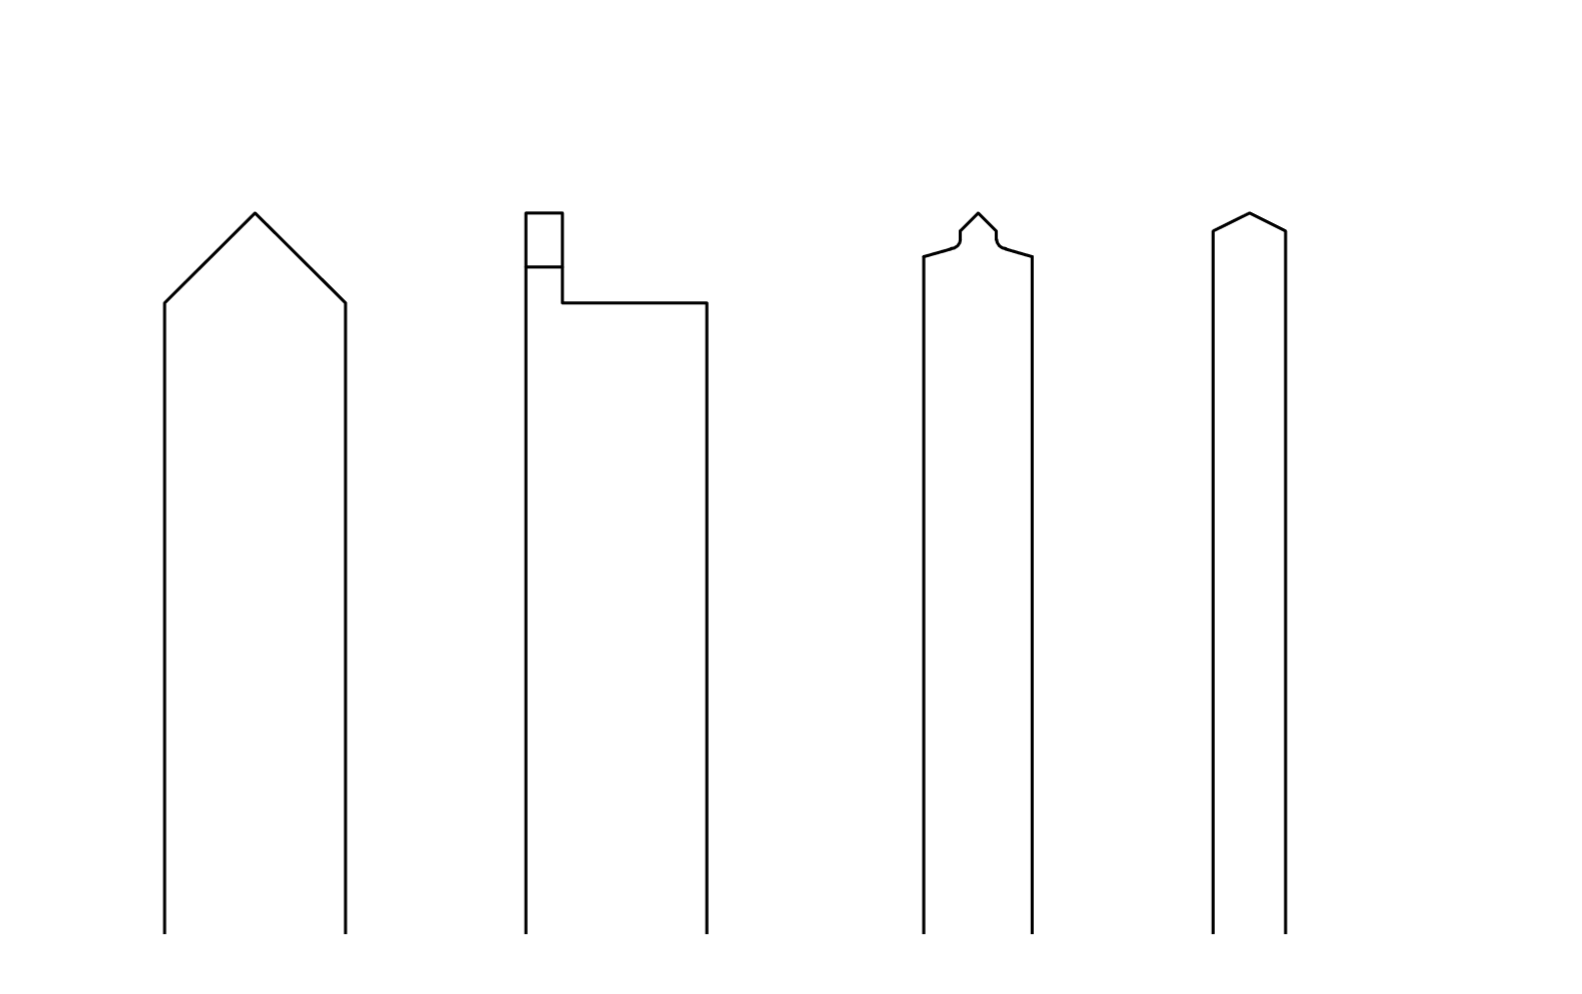
\includegraphics[width=14cm]{skica_orodij.png}
        \caption{Skica orodij
        \cite{lasten}}
        \label{skica_orodij}
    \end{center}
\end{figure}

Te parametre sem približno izbral glede na izkušnje. Ker stroj nima 
menjalnika za hitrost glavnega vretena, sem izbrali enotno hitrost 
2000 \( \frac{vrt}{min} \). Za svedre sem pa uporabil posebnost tega stroja,
da lahko svedre posebej vrti v nasprotno smer od glavnega vretena kar pomeni,
da se hitrosti vrtenja seštevajo in tako lahko dosežemo veliko večje hitrosti 
z manjšo obrabo stroja. To pomeni, da se morajo svedri vrteti z hitrostjo
2200 \( \frac{vrt}{min} \). Za povrtavanje luknje iz druge strani, pa stroj 
kos preprime z posebnim držalom, ki se ne more vrteti, zato sem uporabil največjo
hitrost gnanega orodja; 2200 \( \frac{vrt}{min} \).

Ker nam stroj na krivulje omogoča več obdelav naenkrat bom združil 
struženje prvega in zadnjega roba skupaj z povrtavanjem prejšnjega 
kosa in povrtavanje trenutnega kosa. Z tem lahko čas cikla močno 
zmanjšamo na približno 6-8 s.

\newpage